\documentclass[conference]{IEEEtran}
\usepackage[utf8]{inputenc}
\usepackage[T1]{fontenc}
\usepackage{amsmath,amssymb}
\usepackage{graphicx}
\usepackage{booktabs}
\usepackage{url}
\usepackage{cite}
\usepackage{tikz}
\usetikzlibrary{arrows.meta,positioning}
\graphicspath{{../results/figures/}}
\newcommand{\tab}[1]{\input{../results/tables/#1.tex}}
\newcommand{\factnrows}{504}
\newcommand{\facttargetmedian}{18}
\newcommand{\facttargetmax}{320}
\newcommand{\factfeaturesproc}{DBO-E (20), DQO-E (20), DBO-D (20), DQO-D (20), SED-P (16), DBO-P (14), SS-D (8), SED-E (2)}
\newcommand{\factrmsemglprocfull}{6.05}
\newcommand{\factrmsemglprocanfis}{5.95}
\newcommand{\factrmsemglprocridge}{5.78}
\newcommand{\factrmsemglprocmean}{6.64}
\newcommand{\factfullvsridgeproc}{-0.075}
\newcommand{\factfullvsridgepproc}{0.023}
\newcommand{\factfullvsanfisproc}{-0.029}
\newcommand{\factfullvsanfispproc}{0.365}
\newcommand{\factfullvsanfiswproc}{0.070}
\newcommand{\factfeaturessoft}{DQO-E (20), DBO-D (20), DQO-D (20), DQO-S (20), SS-S (20), DBO-E (18), SED-P (1), PH-S (1)}
\newcommand{\factrmsemglsoftfull}{4.34}
\newcommand{\factrmsemglsoftanfis}{4.35}
\newcommand{\factrmsemglsoftridge}{4.30}
\newcommand{\factrmsemglsoftmean}{6.64}
\newcommand{\factfullvsridgesoft}{-0.009}
\newcommand{\factfullvsridgepsoft}{0.379}
\newcommand{\factfullvsanfissoft}{+0.003}
\newcommand{\factfullvsanfispsoft}{0.899}
\newcommand{\factfullvsanfiswsoft}{0.812}
\newcommand{\factysplit}{353/76/75}
\newcommand{\factyclipmax}{36.5}
\newcommand{\factsanityanfis}{0.948}
\newcommand{\factsanityridge}{0.715}
\newcommand{\factsanitysomp}{0.087}
\newcommand{\factsanitysomd}{+0.007}
\newcommand{\factsanitypsod}{-0.021}
\newcommand{\factsanitypsop}{0.056}

\newcommand{\Rsq}{$R^2$}

\begin{document}

\title{Re-implementing and Stress-Testing an Attention-Infused Parallel ANFIS for Effluent BOD Prediction on Public Wastewater Data}

\author{\IEEEauthorblockN{Jack Emre Flett}
\IEEEauthorblockA{Department of Computer Engineering, Istanbul University-Cerrahpa\c{s}a, Istanbul, T\"urkiye\\
Fuzzy Logic (Bulan{\i}k Mant{\i}k) term project, November 2026}}

\maketitle

\begin{abstract}
Ramya et al.\ (2025) propose a multi-stage neuro-fuzzy framework for predicting effluent biochemical oxygen demand (BOD) in a wastewater treatment plant: a self-organising map (SOM) initialises the membership functions of an adaptive neuro-fuzzy inference system (ANFIS), particle swarm optimisation (PSO) tunes them, three attention modules re-weight features, membership functions and rules, and three ANFIS models run in parallel (PANFIS). They report that every stage raises the test \Rsq{}, from 0.884 to 0.987. Their data and code are not public. This project re-implements the fuzzy part of the framework from scratch in PyTorch and evaluates it on the public UCI Water Treatment Plant dataset with a leakage-free pipeline, 20 repeated splits and paired significance tests. The implementation is validated on a synthetic benchmark, where the ANFIS reaches \Rsq{} = \factsanityanfis{} against \factsanityridge{} for a linear model. On the real data the reported progression does not appear: no stage produces a statistically significant gain, and all six fuzzy models are statistically indistinguishable from, or worse than, ridge regression. As an extension, an ablation of the three attention levels, a parameter-matched control for PANFIS, a validation-based PSO fitness and a noise-robustness test are carried out. None of the added components is shown to matter on this dataset; an equal-weight PANFIS without attention matches the full model with 93\% fewer parameters. The report also documents internal inconsistencies in the reference paper's reported numbers.
\end{abstract}

\begin{IEEEkeywords}
ANFIS, Takagi--Sugeno fuzzy system, self-organising map, particle swarm optimisation, attention, wastewater treatment, reproducibility
\end{IEEEkeywords}

\section{Introduction}
Wastewater treatment plants (WWTPs) must keep the organic load of their effluent below legal limits. The standard indicator, the five-day biochemical oxygen demand (BOD), takes five days to measure in a laboratory, so a plant cannot react to it in time. A model that estimates effluent BOD from quantities that are available earlier would let operators adjust aeration, which is also the largest energy consumer of a plant~\cite{ramya2025}.

The relationship between influent composition, the biological process and effluent quality is non-linear and uncertain, and measurements are noisy and often missing. Fuzzy inference systems are a natural candidate for such problems: they describe the input space with overlapping linguistic regions and attach a simple local model to each region. The adaptive neuro-fuzzy inference system (ANFIS)~\cite{jang1993} makes such a system trainable from data while keeping a rule base that a person can read.

The reference paper of this project, Ramya et al.~\cite{ramya2025}, stacks several extensions on top of ANFIS (Section~\ref{sec:original}) and reports a steady improvement of the test \Rsq{} with each of them on a private dataset of 1,564 samples from a pharmaceutical plant. Neither the data nor the code is available.

\textbf{Scope of this project.} (i) The fuzzy core of the paper is re-implemented from scratch: first-order Takagi--Sugeno ANFIS, SOM initialisation, PSO, GA and ACO tuning, the three attention modules and the parallel ANFIS. The generative AutoGAN pre-processing stage is not a fuzzy component, its scoring formula is not given, and it is replaced by simple statistics (Section~\ref{sec:repro}). (ii) The paper's main experiment, the six-model progression, is repeated on the public UCI Water Treatment Plant dataset~\cite{poch1993}, which the paper itself uses for external validation. (iii) As the original contribution, the experimental design is extended with the controls that the paper lacks: repeated runs with significance tests, an ablation of the attention levels, a parameter-matched control for the parallel architecture, a validation-based PSO fitness and a noise-robustness test. The minimum reproduction requirement adopted for the project is the chain ANFIS $\rightarrow$ SOM-ANFIS $\rightarrow$ SOM-PSO-ANFIS; the attention and parallel models go beyond it.

The aim is to reproduce the paper's \emph{trend}, not its absolute numbers, because the datasets differ. All code, data, raw results and this report are in the project repository.

\section{Related Work}
ANFIS has been applied repeatedly to WWTP modelling. Qiao et al.~\cite{qiao2023} train ANFIS models on operating data of a full-scale plant to predict the removal of COD, BOD, ammonia and suspended solids and report \Rsq{} values above 0.95 for some targets, while noting that identical inputs can map to different outputs, i.e.\ a substantial unexplained variance. Alnajjar and \"U\c{c}\"unc\"u~\cite{alnajjar2022} model the removal efficiency of BOD, total nitrogen, total phosphorus and suspended solids with ANFIS from hydraulic retention time, temperature and dissolved oxygen.

The combination of clustering and ANFIS that the reference paper uses has a close precedent: Mng'ombe et al.~\cite{mngombe2024} compare a plain ANFIS soft sensor for effluent BOD$_5$ with a SOM-assisted one on a sewage plant in Malawi and find the SOM-assisted version better. Metaheuristic tuning of ANFIS is equally common; Ikram et al.~\cite{ikram2024} compare ANFIS tuned with PSO, grey-wolf and gradient-based optimisers for influent total nitrogen.

Non-fuzzy models are strong competitors. Bagherzadeh et al.~\cite{bagherzadeh2021} show on the Melbourne plant data that the choice of input features changes accuracy markedly and that tree ensembles outperform a neural network. Xie et al.~\cite{xie2024} use a hybrid temporal-convolution/LSTM network for hourly effluent nitrogen. Table~\ref{tab:related} summarises these studies. Two patterns are relevant here: almost all report a single train/test split without repeated runs, and very high \Rsq{} values are typically obtained on private data. Nadeau and Bengio~\cite{nadeau2003} show that naive significance tests on repeated random splits are too optimistic and give a corrected test, which is used in this project.

\begin{table}[t]
\caption{Related studies}
\label{tab:related}
\centering
\footnotesize
\begin{tabular}{p{1.55cm}p{2.2cm}p{1.6cm}p{1.9cm}}
\toprule
Study & Method & Target & Data / result \\
\midrule
Ramya et al.~\cite{ramya2025} & SOM-PSO-PANFIS + attention & effluent BOD & private, 1,564 samples; \Rsq{} 0.987 \\
Qiao et al.~\cite{qiao2023} & ANFIS & removal of COD, BOD, NH$_3$, SS & full-scale plant; \Rsq{} $>$ 0.95 for some \\
Mng'ombe et al.~\cite{mngombe2024} & ANFIS vs.\ SOM-assisted ANFIS & effluent BOD$_5$ & one plant; SOM version better \\
Alnajjar, \"U\c{c}\"unc\"u~\cite{alnajjar2022} & ANFIS & BOD, TN, TP, TSS removal & one plant; low MSE \\
Ikram et al.~\cite{ikram2024} & ANFIS + PSO / GWO / GBO & influent TN & one plant; GBO best \\
Bagherzadeh et al.~\cite{bagherzadeh2021} & ANN, RF, GBM + feature selection & influent TN & Melbourne; GBM best \\
Xie et al.~\cite{xie2024} & TCN-LSTM & effluent TN & one plant, hourly \\
\bottomrule
\end{tabular}
\end{table}

\section{Theoretical Background}
\subsection{Fuzzy sets and membership functions}
A fuzzy set $A$ on a universe $X$ is defined by a membership function $\mu_A: X \rightarrow [0,1]$ that states to which degree an element belongs to the set~\cite{zadeh1965}. A linguistic variable such as ``influent BOD'' takes fuzzy sets (``low'', ``high'') as values. This project uses Gaussian membership functions,
\begin{equation}
\mu(x) = \exp\!\left(-\frac{(x-c)^2}{2\sigma^2}\right),
\label{eq:gauss}
\end{equation}
with centre $c$ and width $\sigma$. They are smooth and non-zero everywhere, which is what gradient-based training needs.

\subsection{Mamdani and Sugeno inference}
A fuzzy inference system maps crisp inputs to a crisp output in four steps: fuzzification, rule evaluation, aggregation and defuzzification. In a Mamdani system the consequent of each rule is a fuzzy set, and the aggregated output set is defuzzified, usually by its centroid. In a Takagi--Sugeno (TS) system~\cite{takagi1985} the consequent is a function of the inputs,
\begin{align*}
R_k:\ &\text{IF } x_1 \text{ is } A_{k1} \text{ AND } \dots \text{ AND } x_n \text{ is } A_{kn}\\
&\text{THEN } f_k = a_{k0} + \textstyle\sum_i a_{ki}x_i ,
\end{align*}
and the output is the firing-strength-weighted average of the rule outputs. This weighted average plays the role of defuzzification; no output fuzzy set and no centroid computation are needed, which makes the system differentiable end to end.

\subsection{ANFIS}
ANFIS~\cite{jang1993} writes a first-order TS system as a five-layer network (Fig.~\ref{fig:pipeline}, right):
\begin{align}
\text{L1 (fuzzify):}\quad & \mu_{ki}(x_i) \text{ by (\ref{eq:gauss})} \nonumber\\
\text{L2 (AND, product):}\quad & w_k = \textstyle\prod_{i=1}^{n}\mu_{ki}(x_i) \nonumber\\
\text{L3 (normalise):}\quad & \bar w_k = w_k / \textstyle\sum_{j=1}^{R} w_j \nonumber\\
\text{L4 (consequent):}\quad & \bar w_k f_k,\quad f_k = a_{k0}+\textstyle\sum_i a_{ki}x_i \nonumber\\
\text{L5 (output):}\quad & \hat y = \textstyle\sum_{k=1}^{R}\bar w_k f_k \label{eq:anfis}
\end{align}
The premise parameters $(c_{ki},\sigma_{ki})$ and the consequent parameters $a_{ki}$ are learned from data. For fixed premises the output is linear in the consequents, so they can be obtained by least squares; this is the basis of Jang's hybrid learning and is used here inside the metaheuristic fitness.

\subsection{Self-organising map}
A SOM~\cite{kohonen1990} is a grid of nodes with weight vectors in input space. For each sample the best-matching unit (the closest node) and its grid neighbours are moved towards the sample. After training the nodes are prototypes of the data, and each node can serve as the centre of one fuzzy rule.

\subsection{Metaheuristics}
PSO~\cite{kennedy1995} moves a swarm of candidate solutions through the search space. The velocity of particle $i$ is
\begin{equation}
v_i \leftarrow w v_i + c_1 r_1 (p_i - x_i) + c_2 r_2 (g - x_i),
\end{equation}
where $p_i$ is the particle's best position so far, $g$ the best position of the swarm and $r_1,r_2$ uniform random numbers. A genetic algorithm (GA) evolves a population by selection, crossover and mutation; ant colony optimisation (ACO) guides the search by pheromone values that are reinforced by good solutions and evaporate over time. None of them needs gradients.

\section{Original Method}
\label{sec:original}
The framework of Ramya et al.~\cite{ramya2025} predicts effluent BOD (BODOUT) at the aeration stage from influent and aeration-tank measurements. Its stages are (Fig.~\ref{fig:pipeline}, left):

\emph{1) AutoGAN.} An autoencoder trained adversarially scores the features; those above 0.75 are kept (six of eleven inputs), and samples with a high reconstruction error (79 of 1,564) are replaced by their reconstruction.

\emph{2) SOM initialisation.} SOM node weights become the centres of the Gaussian membership functions, and the widths are derived from the spread of the data (5$\times$5 grid, neighbourhood 0.3, learning rate 0.5, 100 iterations).

\emph{3) Metaheuristic tuning.} GA, ACO and PSO each tune the membership-function parameters with the training MSE as fitness; PSO (50 particles, 40 iterations) is reported as best.

\emph{4) Attention.} Three two-layer networks compute weights: feature attention and membership-function attention with a softmax output, and rule attention with a tanh output so that rules can be suppressed. Their input is the batch average of the corresponding quantity.

\emph{5) Parallel ANFIS.} Three ANFIS models with 9, 16 and 25 rules (SOM grids 3$\times$3, 4$\times$4, 5$\times$5) are trained on the same data and fused.

Training uses Adam (learning rate 0.01, up to 1000 epochs, early stopping), min--max scaling and a 70/15/15 split. Table~\ref{tab:paper} lists the reported progression.

\begin{figure}[t]
\centering
\resizebox{\columnwidth}{!}{%
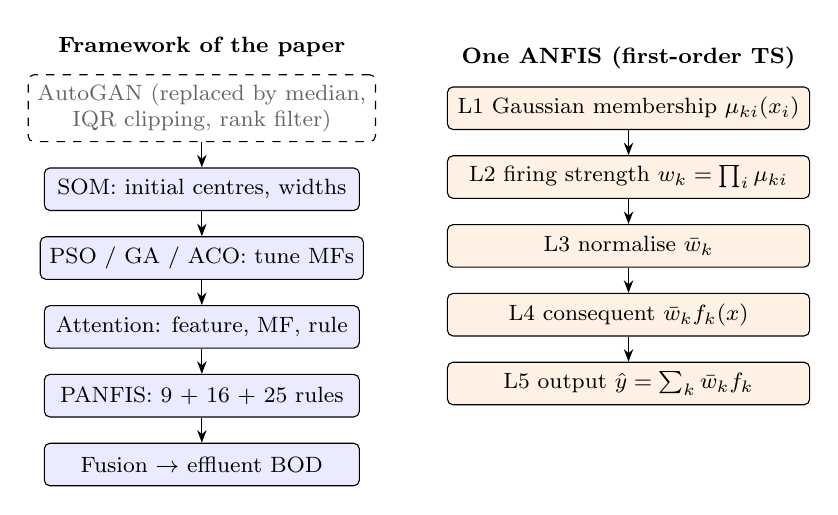
\begin{tikzpicture}[font=\footnotesize, node distance=3.2mm,
  box/.style={draw, rounded corners=2pt, minimum width=40mm, minimum height=5.4mm, align=center},
  ours/.style={box, fill=blue!8}, skip/.style={box, dashed, text=black!60},
  lay/.style={draw, rounded corners=2pt, minimum width=46mm, minimum height=5.4mm, align=center, fill=orange!10},
  arr/.style={-{Stealth[length=1.6mm]}}]
\node[skip] (gan) {AutoGAN (replaced by median,\\ IQR clipping, rank filter)};
\node[ours, below=of gan] (som) {SOM: initial centres, widths};
\node[ours, below=of som] (pso) {PSO / GA / ACO: tune MFs};
\node[ours, below=of pso] (att) {Attention: feature, MF, rule};
\node[ours, below=of att] (pan) {PANFIS: 9 + 16 + 25 rules};
\node[ours, below=of pan] (fus) {Fusion $\rightarrow$ effluent BOD};
\foreach \a/\b in {gan/som, som/pso, pso/att, att/pan, pan/fus} \draw[arr] (\a) -- (\b);
\node[lay, right=9mm of gan] (l1) {L1 Gaussian membership $\mu_{ki}(x_i)$};
\node[lay, below=of l1] (l2) {L2 firing strength $w_k=\prod_i \mu_{ki}$};
\node[lay, below=of l2] (l3) {L3 normalise $\bar w_k$};
\node[lay, below=of l3] (l4) {L4 consequent $\bar w_k f_k(x)$};
\node[lay, below=of l4] (l5) {L5 output $\hat y=\sum_k \bar w_k f_k$};
\foreach \a/\b in {l1/l2, l2/l3, l3/l4, l4/l5} \draw[arr] (\a) -- (\b);
\node[above=1mm of gan] {\textbf{Framework of the paper}};
\node[above=1mm of l1] {\textbf{One ANFIS (first-order TS)}};
\end{tikzpicture}}
\caption{Left: stages of the reference framework; shaded stages are re-implemented, the dashed one is replaced. Right: the five ANFIS layers.}
\label{fig:pipeline}
\end{figure}

\begin{table}[t]
\caption{Test results reported in the reference paper (private data)}
\label{tab:paper}
\centering
\footnotesize
\setlength{\tabcolsep}{3pt}
\begin{tabular}{lcccc}
\toprule
Model & RMSE & SSE & \Rsq{} & $\tfrac{\mathrm{SSE}}{\mathrm{RMSE}^2}$ \\
\midrule
ANFIS & 0.0461 & 0.4987 & 0.8838 & 235 \\
SOM-ANFIS & 0.0393 & 0.3707 & 0.9136 & 240 \\
SOM-PSO-ANFIS & 0.0329 & 0.2538 & 0.9409 & 234 \\
SOM-PSO-ANFIS-Attention & 0.0287 & 0.1937 & 0.9576 & 235 \\
SOM-PSO-PANFIS & 0.0233 & 0.1478 & 0.9751 & 272 \\
SOM-PSO-PANFIS-Attention & 0.0183 & 0.1050 & 0.9866 & 314 \\
\bottomrule
\end{tabular}
\end{table}

\subsection{Critical reading}
\label{sec:critical}
Checking the paper's own numbers against each other reveals several problems. They do not prove that the conclusions are wrong, but they limit how much weight the reported progression can carry.

\emph{Inconsistent metrics.} Since $\mathrm{SSE} = n\cdot\mathrm{RMSE}^2$, the last column of Table~\ref{tab:paper} recovers the test-set size. The first four models give $n\approx235$, which is 15\% of 1,564 as expected; the two PANFIS rows give 272 and 314. Likewise $\mathrm{RMSE}^2/(1-R^2)$, the variance of the test target, should be one constant; it is 0.018 for the first three rows and 0.025 for the last. The two best models were therefore not evaluated on the same test set as the others, or the numbers contain errors.

\emph{Contradictory descriptions.} The third branch has 25 rules in the paper's Table~1, 20 in Section~4.3 and 10 in Section~4.4. Fusion weights are ``equal (1/3 each)'' in Table~1 and Eq.~21 but learned (e.g.\ 47.8/35.9/16.4\%) in the results. In the text, RMSE values are called MAE and MAE values are called SSE. Section~4.2 quotes \Rsq{} 0.906 vs.\ 0.840 for SOM vs.\ uniform initialisation, while its Table~2 gives 0.9136 vs.\ 0.8838. The external validation is said to use the single-ANFIS attention model, but the comparison row for the private data shows the PANFIS-attention numbers.

\emph{Missing controls.} All results are single runs. PANFIS has 50 rules against the 9--25 of a single model, and no single model of equal size is tested, so the effect of the parallel architecture cannot be separated from that of capacity. The attention levels are only tested together.

\emph{Possible leakage.} Scaling and the anomaly replacement are applied to the whole dataset before it is split.

\emph{Unspecified details.} The PSO inertia and acceleration coefficients, the consequents used while the metaheuristics run, the place where attention weights enter the network, and the AutoGAN importance function (its Eq.~10 is only written as $f(\cdot)$) are not given. Because the attention input is a batch average, the prediction for one sample depends on the other samples in the batch.

\section{Reproduction Methodology}
\label{sec:repro}
Everything is implemented in Python with PyTorch for the differentiable parts and NumPy for SOM and the metaheuristics. No external ANFIS code is used.

\subsection{Data and pre-processing}
The UCI Water Treatment Plant dataset~\cite{poch1993} contains 527 daily records (1990--1991) of an urban plant with 38 attributes measured at the plant input (E), the primary settler (P), the secondary settler input (D) and the output (S), plus computed removal efficiencies (RD). The target is the effluent BOD (DBO-S). The \factnrows{} records with a known target are used.

Two input scenarios are defined. \emph{Process inputs}: the 22 upstream attributes (E, P, D), mirroring the paper's ``influent and aeration tank $\rightarrow$ effluent'' setting. \emph{Soft-sensor inputs}: additionally the six fast effluent measurements (pH, COD, solids, conductivity), which are available days before BOD. The RD attributes are never used because they are computed from effluent values, two of them directly from the target.

The split is 70/15/15 (\factysplit{} samples). All statistics come from the training part only: (1) missing values are replaced by training medians; (2) inputs and target are clipped to the Tukey fences $[Q_1-1.5\,\mathrm{IQR},\,Q_3+1.5\,\mathrm{IQR}]$, replacing the AutoGAN anomaly handling; (3) the six inputs with the largest absolute Spearman correlation to the target are kept, replacing the AutoGAN feature selection (the paper also keeps six); (4) inputs and target are min--max scaled. The target has a median of \facttargetmedian{}~mg/L and a maximum of \facttargetmax{}~mg/L on a plant-fault day; because clipping the test target is debatable, results on the unclipped test target are reported as well.

\subsection{ANFIS, SOM and metaheuristics}
The ANFIS follows (\ref{eq:anfis}). Each rule owns one Gaussian per input, so the number of rules equals the number of SOM nodes and does not grow exponentially with the inputs. Firing strengths are computed in log space for numerical stability. A unit test compares the network output with a hand computation of the five layers.

The SOM is implemented as in the paper's Eqs.~5--6. Node weights become centres; the width of rule $k$ for input $i$ is the standard deviation of the training samples mapped to node $k$, limited to $[0.05, 0.5]$. The non-SOM baseline (``uniform initialisation'') draws centres from $[0.1,0.9]$ and widths from $[0.1,0.5]$ as in the paper's Table~1.

PSO, GA and ACO search the $2nR$ membership parameters within $[0,1]$. The fitness of a candidate is the training MSE of the ANFIS whose consequents are obtained by ridge-regularised least squares. Each optimiser starts from the SOM solution. After this stage all parameters are trained with Adam and early stopping on the validation set.

\subsection{Attention and PANFIS}
The scoring networks follow the paper's Eqs.~19--20 (two layers, 16 hidden units). Their placement is this project's design decision, chosen so that every weight has a fuzzy-logic meaning:
\begin{align}
\text{feature:}\ \ & \mu_{ki} \leftarrow \mu_{ki}^{\,n\alpha_i}, && \alpha=\mathrm{softmax}(\cdot) \nonumber\\
\text{MF:}\ \ & \mu_{ki} \leftarrow \mu_{ki}^{\,R\gamma_{ki}}, && \gamma_{\cdot i}=\mathrm{softmax\ over\ rules} \nonumber\\
\text{rule:}\ \ & \bar w_k \leftarrow \bar w_k(1+\beta_k), && \beta=\tanh(\cdot)
\end{align}
An exponent above one sharpens a membership function (the input matters more for the rule), an exponent below one flattens it. The last layer of each scoring network is initialised to zero, so that initially $\alpha_i=1/n$, $\gamma_{ki}=1/R$, $\beta_k=0$ and the model equals the plain ANFIS exactly (verified by a unit test). As in the paper the scorer sees the batch average; with full-batch training this is the training-set average, which is stored and reused at inference so that predictions do not depend on the test batch. A per-sample variant is tested in the extension.

PANFIS trains three branches (9, 16, 25 rules) independently and combines them linearly. Both readings of the paper are implemented: equal weights, and three weights fitted by least squares on the validation predictions.

\subsection{Deviations from the paper}
Table~\ref{tab:dev} lists every choice that is not taken from the paper. The ridge strength was selected on the validation data of five development seeds that are not used for reporting; no choice was tuned on test data.

\begin{table}[t]
\caption{Choices not specified by, or different from, the paper}
\label{tab:dev}
\centering
\footnotesize
\begin{tabular}{p{2.6cm}p{5.2cm}}
\toprule
Item & This project \\
\midrule
Dataset & UCI WWTP (public) instead of the private one \\
AutoGAN & median imputation, IQR clipping, top-6 $|\rho_\text{Spearman}|$ \\
Rules, single model & 9 (3$\times$3 SOM); paper states 9, 10 or 25 \\
SOM ``100 iterations'' & read as 100 passes over the training set \\
PSO coefficients & $w=0.7$, $c_1=c_2=1.5$ (not given) \\
GA mutation $\sigma$ & 0.1 instead of the printed 1 (search space is $[0,1]$) \\
ACO & pheromone as per-parameter step size (paper Eqs.~15--16) \\
Fitness consequents & ridge least squares, $\lambda=0.3$ (not given) \\
Early stopping & patience 50; LR halved after 20 stagnant epochs \\
Attention placement & exponents on $\mu$, factor on $\bar w$ (not given) \\
Attention input & stored training average at inference \\
\bottomrule
\end{tabular}
\end{table}

\section{Proposed Extension}
The contribution of this project is experimental: it supplies the controls whose absence was noted in Section~\ref{sec:critical} and tests whether the paper's claims hold under them.

\emph{E0: Repeated evaluation with significance tests.} Every model is trained 20 times on different random splits and initialisations. Models are compared pairwise on identical splits and identical SOM/PSO starting points, so that only the component under test differs. Significance is assessed with the corrected resampled $t$-test~\cite{nadeau2003}, $t = \bar d / \sqrt{(1/k + n_\text{test}/n_\text{train})\,s_d^2}$, which accounts for the overlap between repeated splits. A second protocol uses one chronological split (train on the past, test on the future) with ten initialisations.

\emph{E1: Attention ablation.} SOM-PSO-ANFIS is trained with every subset of the three attention levels, and with a per-sample variant of the full attention. \emph{Rationale:} the paper only tests all three together, so the contribution of each level is unknown.

\emph{E2: Parameter-matched control.} PANFIS (9+16+25 rules, 950 parameters) is compared with a single ANFIS with 50 rules (5$\times$10 SOM, also 950 parameters), with single models of 9, 16 and 25 rules, with equal instead of learned fusion weights and with a homogeneous 16+16+16 ensemble. \emph{Rationale:} to separate the effect of the parallel architecture from that of model size, and to resolve the paper's equal-vs-learned contradiction empirically.

\emph{E3: Validation-based PSO fitness.} The paper's fitness is the training MSE, which rewards memorisation. The variant fits the consequents on the training set but measures the fitness on the validation set.

\emph{E4: Noise robustness and non-fuzzy baselines.} Gaussian noise of increasing standard deviation is added to the test inputs of trained models. Ridge regression, a multilayer perceptron and a random forest serve as references. \emph{Rationale:} robustness to sensor noise is a main argument for fuzzy models, and the paper compares only against an LSTM.

\emph{E5: Synthetic sanity check.} The whole pipeline is run on the Friedman~\#1 function with 1,564 samples, to verify the implementation independently of the wastewater data.

\section{Experimental Setup}
\textbf{Software:} Python 3.13, PyTorch 2.15, NumPy 2.5, scikit-learn 1.9, SciPy 1.18, Matplotlib 3.11 (exact versions in \texttt{requirements.txt}). \textbf{Hardware:} two CPU cores of a cloud Linux machine, no GPU; the complete study runs in about 30 minutes. \textbf{Hyper-parameters:} as in the paper's Table~1 where given (Section~\ref{sec:original}), otherwise as in Table~\ref{tab:dev}. \textbf{Protocols:} 20 random 70/15/15 splits (seeds 0--19) and one chronological split with 10 initialisations, each for both input scenarios. \textbf{Metrics:} MSE, RMSE, MAE, SSE and \Rsq{} on the scaled target as in the paper, plus RMSE in mg/L. \textbf{Baselines:} mean predictor, ridge regression ($\lambda=1$), MLP (32-16, early stopping), random forest (300 trees). Over the 20 splits the selected process inputs were \factfeaturesproc{} (number of splits in parentheses) and the soft-sensor inputs \factfeaturessoft{}.

\section{Results}
\subsection{Implementation check on synthetic data}
On the synthetic benchmark (Table~\ref{tab:sanity}) the plain ANFIS reaches \Rsq{} = \factsanityanfis{}, close to the noise ceiling of about 0.96 and far above ridge regression (\factsanityridge). The implementation therefore learns non-linear structure when it exists. SOM initialisation changes \Rsq{} by \factsanitysomd{} ($p=$ \factsanitysomp) and PSO by \factsanitypsod{} ($p=$ \factsanitypsop); even here the later stages add little.

\begin{table}[t]
\caption{Synthetic benchmark (Friedman \#1, 10 repetitions, test set)}
\label{tab:sanity}
\centering
\resizebox{\columnwidth}{!}{\tab{sanity_synthetic}}
\end{table}

\subsection{Reproduction of the model progression}
Tables~\ref{tab:ladderproc} and~\ref{tab:laddersoft} and Fig.~\ref{fig:ladder} show the main experiment. The column $\Delta R^2$ is the mean paired change with respect to the previous model of the progression (for GA and ACO: with respect to SOM-ANFIS).

\begin{table*}[t]
\caption{Process inputs: test metrics on the scaled target, mean $\pm$ std over 20 random splits. $p$: corrected resampled $t$-test of $\Delta R^2$}
\label{tab:ladderproc}
\centering
\footnotesize
\tab{ladder_process}
\end{table*}

\begin{table*}[t]
\caption{Soft-sensor inputs: test metrics on the scaled target, mean $\pm$ std over 20 random splits}
\label{tab:laddersoft}
\centering
\footnotesize
\tab{ladder_softsensor}
\end{table*}

\begin{figure*}[t]
\centering
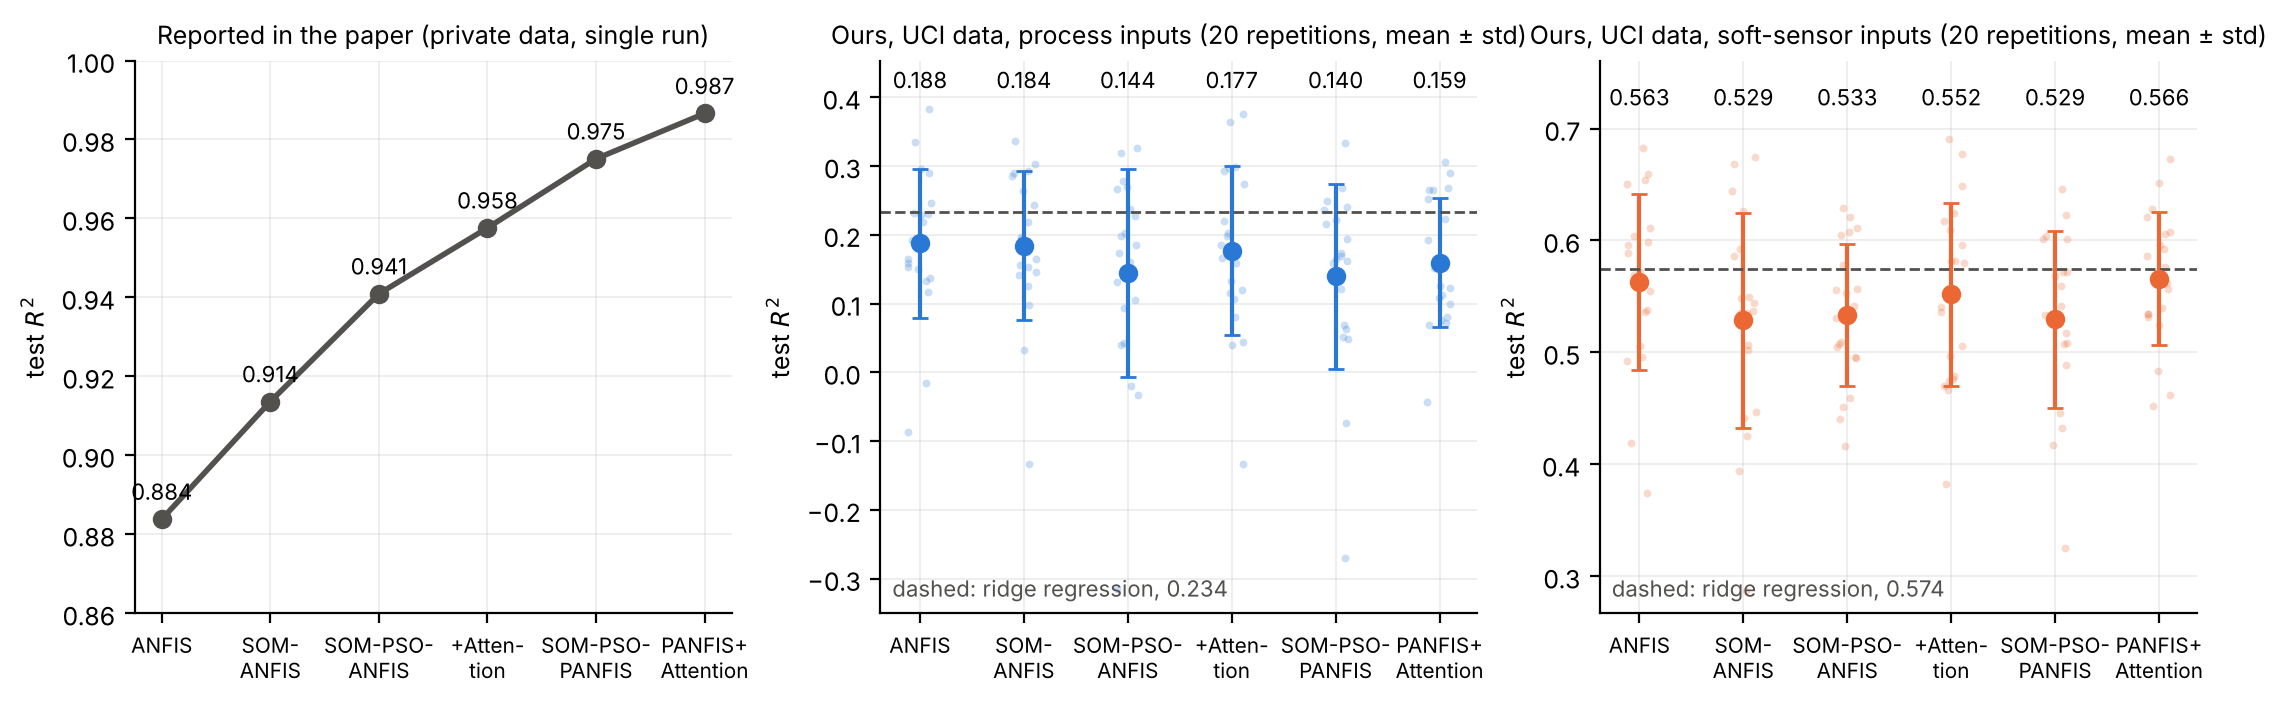
\includegraphics[width=\textwidth]{ladder.png}
\caption{Model progression. Left: values reported in the paper. Centre and right: this project, UCI data; small dots are single repetitions, large dots with bars are mean $\pm$ std.}
\label{fig:ladder}
\end{figure*}

\emph{The progression is not reproduced.} With process inputs the test \Rsq{} lies between 0.14 and 0.19 for all six fuzzy models, with a standard deviation of about 0.1 across splits. No step of the progression is significant ($p \geq 0.19$), and the signs alternate. The full model differs from the plain ANFIS by \factfullvsanfisproc{} ($p=$ \factfullvsanfispproc). With soft-sensor inputs all models lie between 0.53 and 0.57 and again no step is significant; the full model differs from the plain ANFIS by \factfullvsanfissoft{} ($p=$ \factfullvsanfispsoft).

\emph{Fuzzy models do not beat a linear model.} Ridge regression with seven parameters is at least as accurate as every fuzzy model in both scenarios. With process inputs the full model (13,238 parameters) is worse than ridge by \factfullvsridgeproc{} in \Rsq{} ($p=$ \factfullvsridgepproc); with soft-sensor inputs the difference is \factfullvsridgesoft{} ($p=$ \factfullvsridgepsoft). In physical units the test RMSE is \factrmsemglprocridge{}~mg/L (ridge) vs.\ \factrmsemglprocfull{}~mg/L (full model) for process inputs and \factrmsemglsoftridge{} vs.\ \factrmsemglsoftfull{}~mg/L for soft-sensor inputs; predicting the training mean gives \factrmsemglprocmean{}~mg/L.

\emph{Metaheuristics.} PSO lowers the training fitness faster than GA and ACO (Fig.~\ref{fig:conv}), in line with the paper, but this does not carry over to the test set: none of the three improves on SOM-ANFIS significantly.

\emph{Absolute level.} The paper reports \Rsq{} = 0.85--0.87 for its single-ANFIS attention model on this dataset without stating inputs or pre-processing. This project obtains 0.18 (process) and 0.55 (soft sensor) for the same model. Table~\ref{tab:chrono} shows that the picture is the same or worse on the unclipped test target and on the chronological split, where process-input models barely beat the mean predictor.

\begin{table}[t]
\caption{Test $R^2$: mean on the unclipped (raw) test target over the 20 random splits, and mean $\pm$ std on the chronological split (10 initialisations)}
\label{tab:chrono}
\centering
\footnotesize\setlength{\tabcolsep}{2pt}\resizebox{\columnwidth}{!}{\tab{ladder_chrono_raw}}
\end{table}

\begin{figure}[t]
\centering
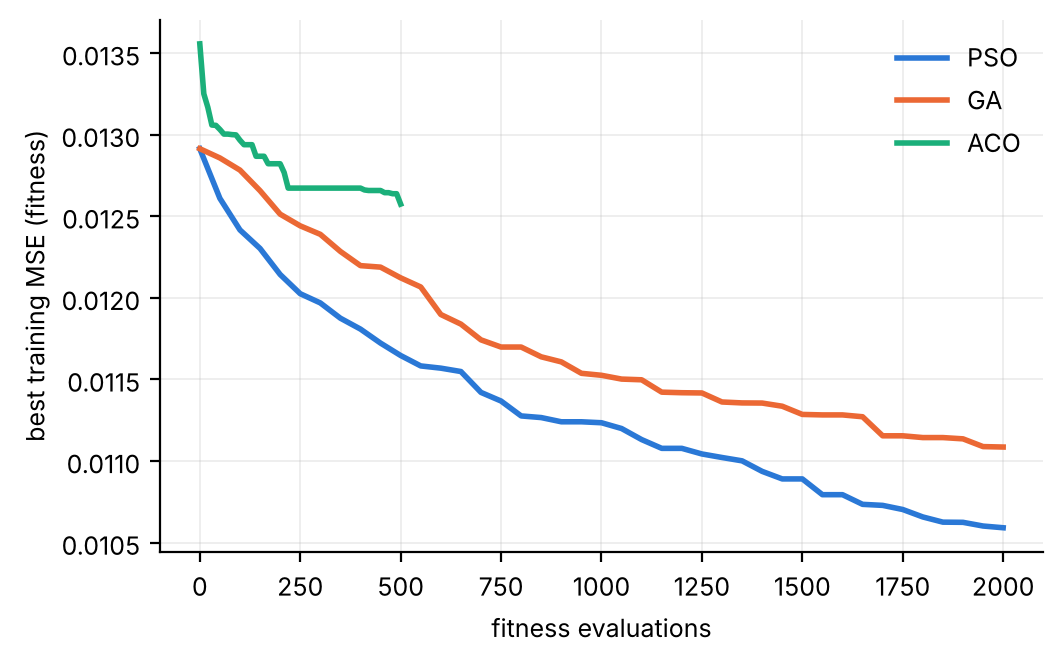
\includegraphics[width=0.8\columnwidth]{convergence.png}
\caption{Best training fitness of the three metaheuristics against the number of fitness evaluations (soft-sensor inputs, mean of 5 seeds).}
\label{fig:conv}
\end{figure}

\begin{figure*}[t]
\centering
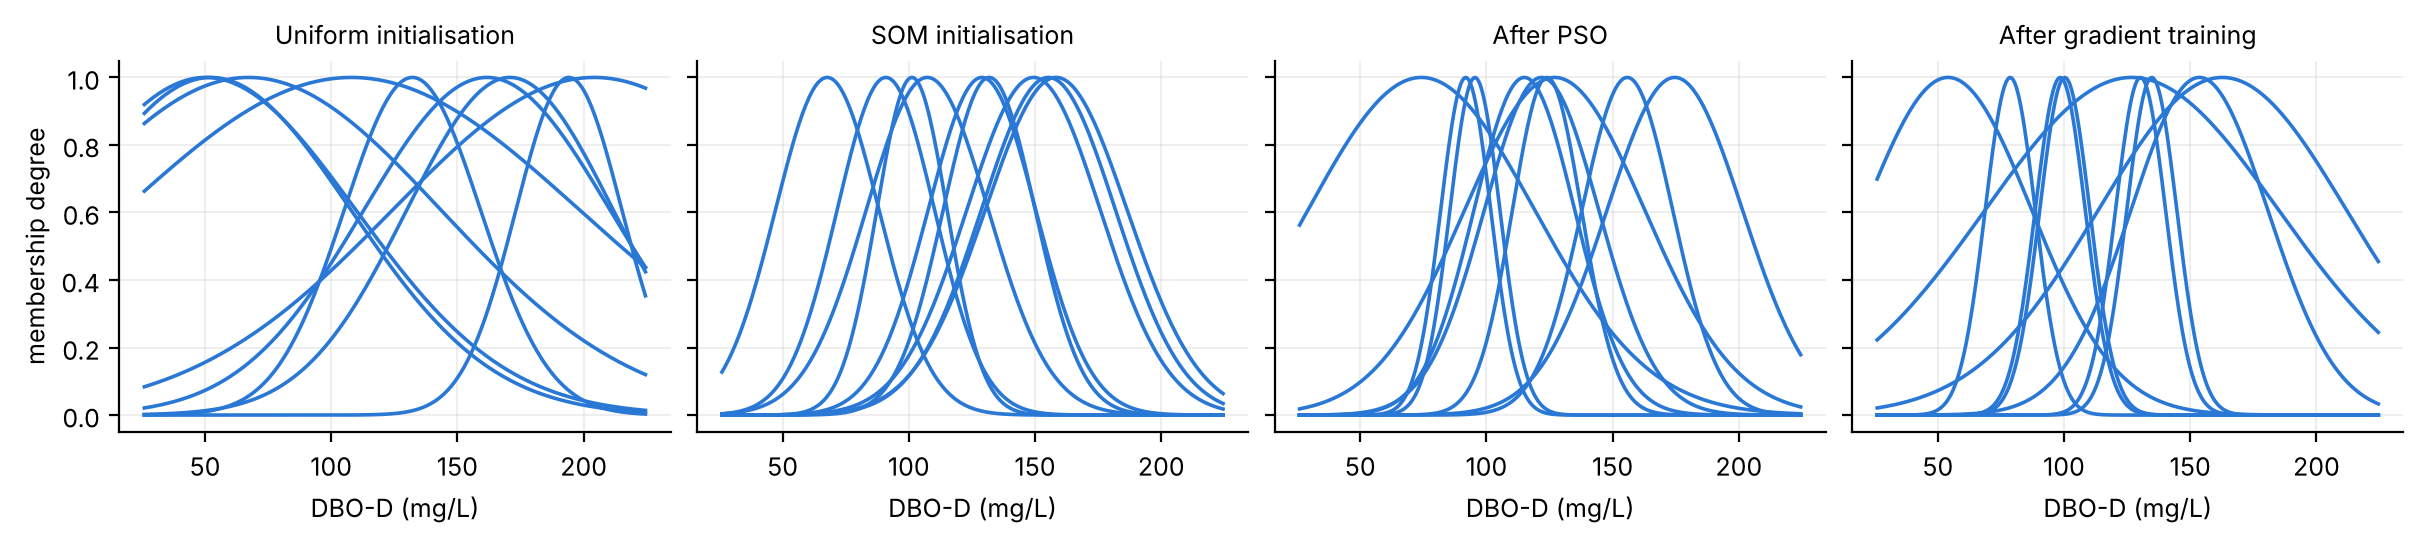
\includegraphics[width=\textwidth]{membership_stages.png}
\caption{Membership functions of one input (BOD at the secondary settler input) of the nine rules at four stages of the pipeline (seed 0, soft-sensor inputs).}
\label{fig:mf}
\end{figure*}

\begin{figure*}[t]
\centering
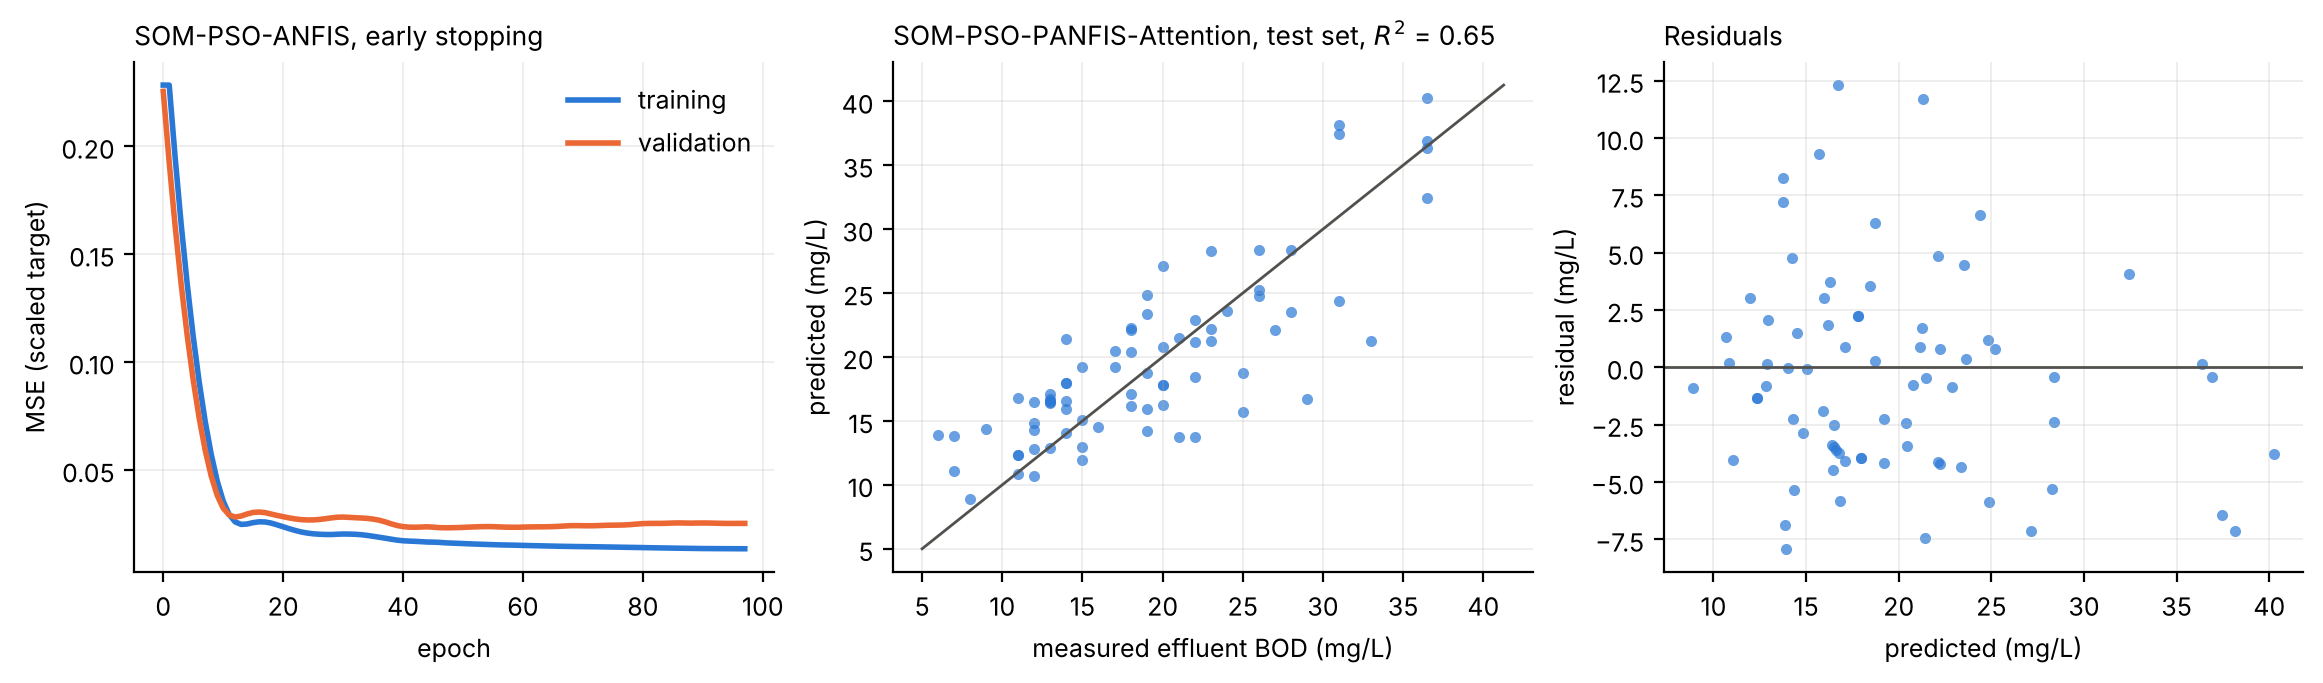
\includegraphics[width=\textwidth]{training_and_predictions.png}
\caption{Left: training and validation loss. Centre and right: predictions and residuals of the full model on the test set (seed 0, soft-sensor inputs).}
\label{fig:pred}
\end{figure*}

\subsection{E1: Attention ablation}
Table~\ref{tab:abl} and Fig.~\ref{fig:abl} give the effect of each attention subset relative to the same model without attention. All confidence intervals include zero. The largest mean changes are $+0.045$ (MF attention, process inputs) and $-0.023$ (rule attention, soft-sensor inputs), both far from significant. The per-sample variant is not better than the paper's batch-average variant. Full attention multiplies the number of parameters by 15 (171 $\rightarrow$ 2,496).

\begin{table*}[t]
\caption{E1: attention ablation on SOM-PSO-ANFIS (F = feature, M = membership function, R = rule). $\Delta$ and $p$ relative to ``none''}
\label{tab:abl}
\centering
\footnotesize
\tab{ablation}
\end{table*}

\begin{figure}[t]
\centering
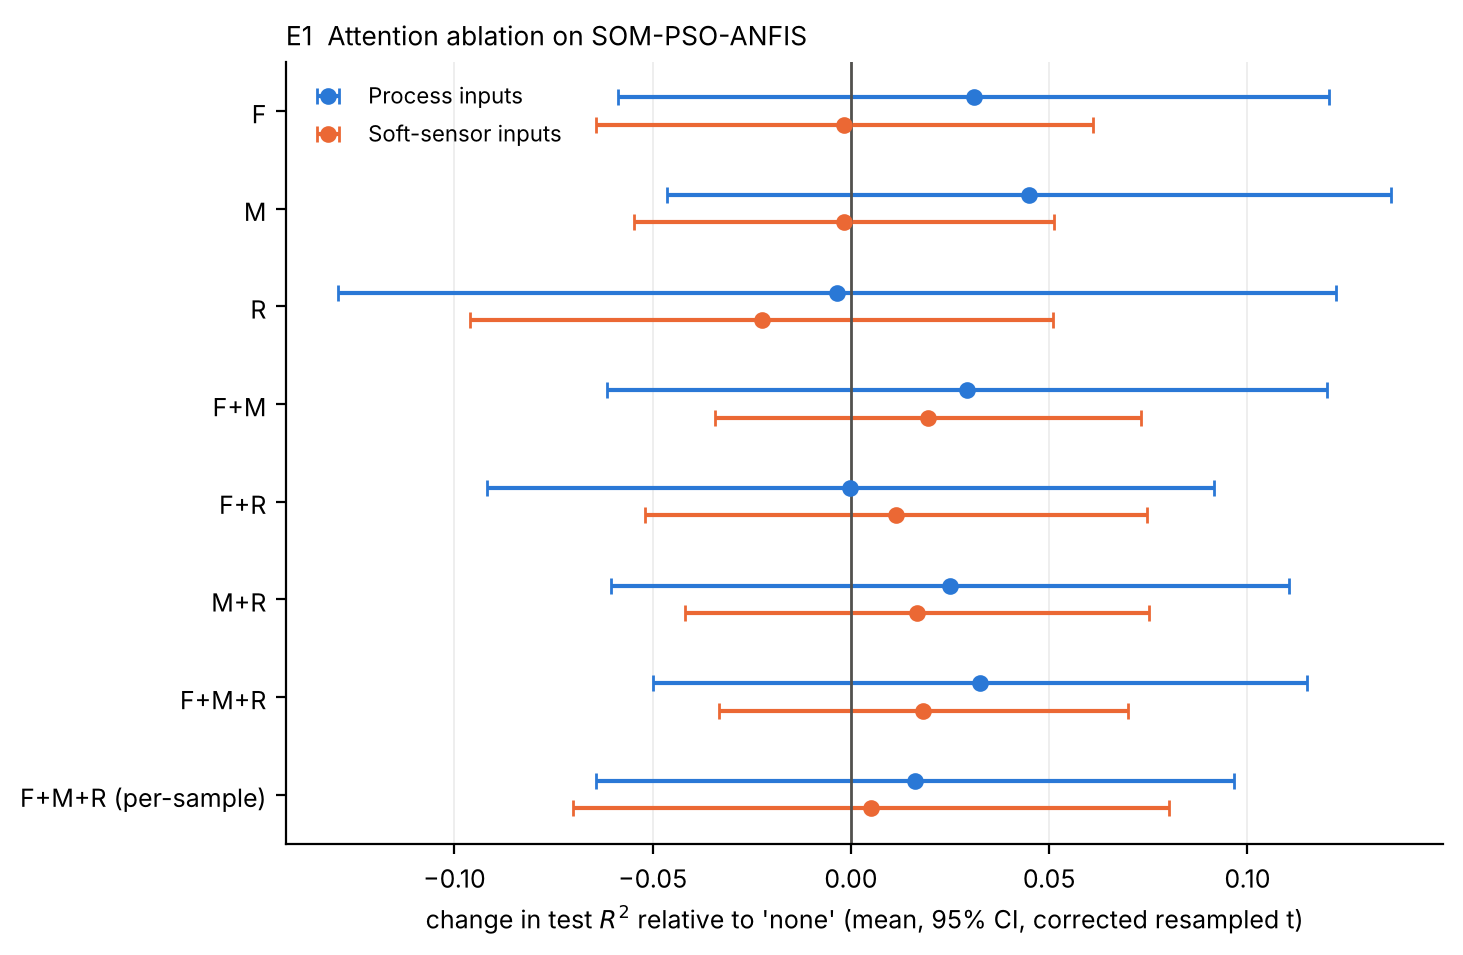
\includegraphics[width=\columnwidth]{ablation.png}
\caption{E1: change in test $R^2$ caused by each attention subset.}
\label{fig:abl}
\end{figure}

\subsection{E2: Is PANFIS more than ``more rules''?}
Table~\ref{tab:struct} compares structures. The single ANFIS with 50 rules, which has exactly the parameter count of PANFIS, is slightly worse than PANFIS in both scenarios ($-0.016$ and $-0.040$), but not significantly. Single models with 9 to 25 rules are on par with PANFIS. Equal fusion weights are slightly better than learned ones in both scenarios ($+0.032$, $+0.020$), which is plausible because three more weights are fitted on only 76 validation samples. The heterogeneous 9+16+25 design shows no advantage over three 16-rule branches.

\begin{table*}[t]
\caption{E2: structure control (all SOM + PSO, no attention). $\Delta$ and $p$ relative to PANFIS 9+16+25 with learned fusion}
\label{tab:struct}
\centering
\footnotesize
\tab{structure}
\end{table*}

\subsection{E3: PSO fitness}
Measuring the PSO fitness on the validation set instead of the training set changes test \Rsq{} by $+0.025$ (process) and $+0.000$ (soft sensor), neither significant (Table~\ref{tab:fit}). Leaving PSO out altogether is as good as either variant.

\begin{table*}[t]
\caption{E3: fitness of the PSO stage. $\Delta$ and $p$ relative to the paper's choice}
\label{tab:fit}
\centering
\footnotesize
\tab{fitness}
\end{table*}

\subsection{E4: Noise robustness}
Fig.~\ref{fig:noise} shows test \Rsq{} under input noise. Up to a noise level of 5\% of the input range all models lose less than 0.03. At 20\% the fuzzy models lose 0.07--0.08 with process inputs, less than ridge regression ($-0.13$) and the MLP ($-0.14$), because they start lower; in absolute terms the plain ANFIS and ridge end at the same level (0.11). With soft-sensor inputs all models degrade alike ($-0.19$ to $-0.25$), the MLP most. There is no evidence that attention or the parallel structure improves robustness.

\begin{figure*}[t]
\centering
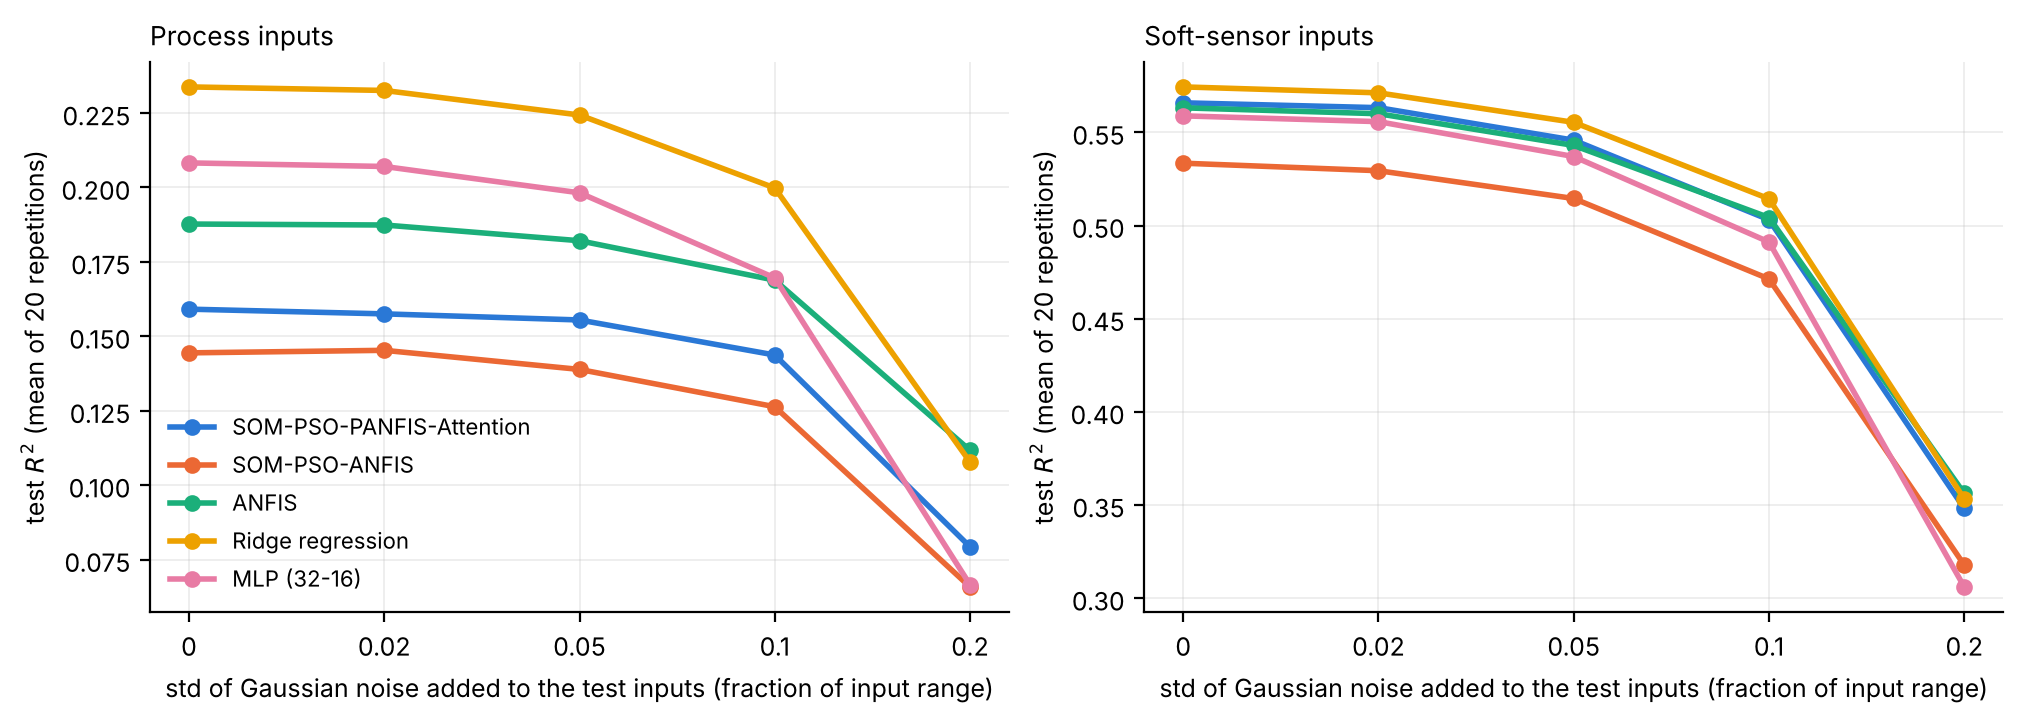
\includegraphics[width=0.9\textwidth]{noise.png}
\caption{E4: test $R^2$ when Gaussian noise is added to the test inputs.}
\label{fig:noise}
\end{figure*}

\subsection{Baseline vs.\ simplified model}
Table~\ref{tab:summary} compares the paper's final architecture with the simplest ensemble suggested by E1 and E2: PANFIS with equal fusion weights and no attention. Accuracy is the same within noise, with 93\% fewer parameters. Training time is dominated by the three PSO runs and hardly changes.

\begin{table}[t]
\caption{Paper's final architecture (baseline) vs.\ equal-weight PANFIS without attention (simplified), means over 20 splits}
\label{tab:summary}
\centering
\resizebox{0.95\columnwidth}{!}{\tab{summary_baseline_vs_proposed}}
\end{table}

\section{Discussion}
\textbf{Why does the progression not appear?} Three explanations are consistent with the evidence. First, the UCI data contain little non-linear signal that the six selected inputs can explain: a linear model is as good as any other model tried, including a random forest. When the mapping is essentially linear plus noise, better membership functions cannot help, since a first-order TS system already contains the linear model as a special case. Second, the dataset is small: 353 training samples against 171 to 13,238 parameters. Early stopping ends training after roughly 100 epochs, before the membership functions have moved far from their initial values (Fig.~\ref{fig:mf}), so the initialisation method and the metaheuristic matter little. PSO does lower the training error (Fig.~\ref{fig:conv}), which is exactly what it optimises, but this is not generalisation. Third, differences of the size reported in the paper (0.01--0.03 in \Rsq{}) are far below the split-to-split standard deviation observed here (0.06--0.15). A single run cannot resolve them; with 20 repetitions and a corrected test, effects of about $\pm0.05$--$0.1$ could not be detected in this study either.

\textbf{What the synthetic check adds.} On data with a known smooth non-linearity and four times as many samples, the same code is far better than a linear model. The negative result on the UCI data is therefore a property of the data and the evaluation protocol, not of a broken implementation. Even there, however, SOM and PSO add at most 0.01, so the large stage-wise gains of the paper are not a generic property of the method.

\textbf{Relation to the paper's claims.} This project cannot test the paper's results on its private data. It does show that (i) the claimed stage-wise improvements do not transfer to the public dataset that the paper uses for external validation; (ii) the \Rsq{} of 0.85--0.87 reported there could not be approached with a leakage-free pipeline, with either input scenario; (iii) the paper's own tables are internally inconsistent for precisely the two best models (Section~\ref{sec:critical}). A plausible contributor to the gap is pre-processing fitted on the full dataset, in particular an anomaly replacement that also smooths the test targets.

\textbf{Interpretability.} A practical benefit of the fuzzy model survives: every prediction can be traced to a few rules with readable centres in mg/L and a local linear model, which the demonstration script prints. This benefit belongs to the plain nine-rule ANFIS. The attention networks add thousands of parameters without measurable gain and make the rule base harder to read.

\section{Limitations}
(1) The private dataset of the paper is unavailable, so the comparison is between trends, not numbers. (2) AutoGAN was replaced by simple statistics; a learned feature selection might choose better inputs. (3) Several details had to be filled in (Table~\ref{tab:dev}); other choices, especially for the attention placement, might behave differently. (4) Only six inputs are used, as in the paper; models with all inputs were not explored. (5) The dataset is small and from one plant in 1990--1991; test sets of 75 samples make every estimate noisy, and the statistical power of the study is limited. (6) The chronological results depend on a single split. (7) Hyper-parameters were not tuned per model; the paper's values were used. (8) The validation set is used for early stopping, for the fusion weights and, in E3, for the PSO fitness, so validation scores are optimistic; all conclusions are based on test scores. (9) GA and ACO receive different evaluation budgets (2,000 and 500), as in the paper.

\section{Conclusion}
The fuzzy core of the attention-infused parallel ANFIS framework of Ramya et al.\ was re-implemented from scratch and evaluated on public wastewater data with repeated, leakage-free experiments. The implementation is correct on a synthetic benchmark, but on the UCI Water Treatment Plant data none of the stages (SOM initialisation, PSO, attention, parallel models) yields a statistically significant improvement, and a ridge regression with seven parameters is as accurate as the full model with over thirteen thousand. The extension experiments show that no single attention level matters, that the parallel architecture is not distinguishable from single models of similar or smaller size, that equal fusion weights are sufficient and that the choice of PSO fitness is immaterial on this dataset. Together with the inconsistencies found in the paper's tables, this suggests that the reported monotone progression should be treated with caution until it is confirmed with repeated runs on shared data.

Future work: obtain the authors' data or the Melbourne plant dataset to test whether the stages help when more samples and stronger non-linearity are available; use time-lagged inputs, since the plant has a retention time of several hours to days; compare Gaussian with other membership functions and a zero-order (constant-consequent) system, which has fewer parameters; and study type-2 fuzzy sets for the measurement uncertainty.

\section*{Generative AI Usage Disclosure}
Generative AI was used extensively in this project. Anthropic's Claude was used (a) to analyse the reference paper and to check its reported numbers for consistency, (b) to explain the theoretical background to the author, (c) to write the source code, the unit tests and the experiment scripts, and to run the experiments, (d) to search for related literature, and (e) to draft this report, the README and the presentation. Every commit that contains AI-written code is marked with a \texttt{Co-Authored-By} line in the Git history. All numerical results in this report were produced by running the code in the repository; no result was generated or estimated by the AI model, and all tables are generated directly from the raw result files. Every reference was checked against the publisher's or repository's page (see \texttt{references/README.md}). The author has read and run the code, checked the results and takes responsibility for the content.

\begin{thebibliography}{00}
\bibitem{ramya2025} S. Ramya, S. Srinath, P. Tuppad, and V. Chandan, ``An attention infused multi-stage parallel adaptive neuro fuzzy systems framework with metaheuristic optimization for accurate water quality prediction,'' \emph{Discover Artif. Intell.}, vol. 5, Art. no. 359, 2025, doi: 10.1007/s44163-025-00624-y.
\bibitem{jang1993} J.-S. R. Jang, ``ANFIS: adaptive-network-based fuzzy inference system,'' \emph{IEEE Trans. Syst., Man, Cybern.}, vol. 23, no. 3, pp. 665--685, 1993, doi: 10.1109/21.256541.
\bibitem{poch1993} M. Poch, ``Water Treatment Plant,'' UCI Machine Learning Repository, 1993, doi: 10.24432/C5FS4C.
\bibitem{qiao2023} L. Qiao \emph{et al.}, ``Exploring ANFIS application based on actual data from wastewater treatment plant for predicting effluent removal quality of selected major pollutants,'' \emph{J. Water Process Eng.}, vol. 56, Art. no. 104247, 2023, doi: 10.1016/j.jwpe.2023.104247.
\bibitem{alnajjar2022} H. Y. H. Alnajjar and O. \"U\c{c}\"unc\"u, ``Enhance modelling predicting for pollution removal in wastewater treatment plants by using an adaptive neuro-fuzzy inference system,'' \emph{Environ. Res. Technol.}, vol. 5, no. 3, 2022.
\bibitem{mngombe2024} M. H. Mng'ombe, E. W. Mtonga, B. A. Chunga, R. C. G. Chidya, and M. Malota, ``Comparative study for the performance of pure artificial intelligence software sensor and self-organizing map assisted software sensor in predicting 5-day biochemical oxygen demand for Kauma Sewage Treatment Plant effluent in Malawi,'' \emph{Front. Environ. Eng.}, vol. 3, Art. no. 1373881, 2024, doi: 10.3389/fenve.2024.1373881.
\bibitem{ikram2024} M. Ikram \emph{et al.}, ``Enhancing the prediction of influent total nitrogen in wastewater treatment plant using adaptive neuro-fuzzy inference system--gradient-based optimization algorithm,'' \emph{Water}, vol. 16, no. 21, Art. no. 3038, 2024, doi: 10.3390/w16213038.
\bibitem{bagherzadeh2021} F. Bagherzadeh, M.-J. Mehrani, M. Basirifard, and J. Roostaei, ``Comparative study on total nitrogen prediction in wastewater treatment plant and effect of various feature selection methods on machine learning algorithms performance,'' \emph{J. Water Process Eng.}, vol. 41, Art. no. 102033, 2021, doi: 10.1016/j.jwpe.2021.102033.
\bibitem{xie2024} Y. Xie, Y. Chen, Q. Wei, and H. Yin, ``A hybrid deep learning approach to improve real-time effluent quality prediction in wastewater treatment plant,'' \emph{Water Res.}, vol. 250, Art. no. 121092, 2024, doi: 10.1016/j.watres.2023.121092.
\bibitem{nadeau2003} C. Nadeau and Y. Bengio, ``Inference for the generalization error,'' \emph{Mach. Learn.}, vol. 52, pp. 239--281, 2003, doi: 10.1023/A:1024068626366.
\bibitem{zadeh1965} L. A. Zadeh, ``Fuzzy sets,'' \emph{Inf. Control}, vol. 8, no. 3, pp. 338--353, 1965, doi: 10.1016/S0019-9958(65)90241-X.
\bibitem{takagi1985} T. Takagi and M. Sugeno, ``Fuzzy identification of systems and its applications to modeling and control,'' \emph{IEEE Trans. Syst., Man, Cybern.}, vol. SMC-15, no. 1, pp. 116--132, 1985, doi: 10.1109/TSMC.1985.6313399.
\bibitem{kohonen1990} T. Kohonen, ``The self-organizing map,'' \emph{Proc. IEEE}, vol. 78, no. 9, pp. 1464--1480, 1990, doi: 10.1109/5.58325.
\bibitem{kennedy1995} J. Kennedy and R. Eberhart, ``Particle swarm optimization,'' in \emph{Proc. ICNN'95 -- Int. Conf. Neural Netw.}, vol. 4, 1995, pp. 1942--1948, doi: 10.1109/ICNN.1995.488968.
\end{thebibliography}

\end{document}
